\documentclass[a4paper,twoside,11pt,chapterprefix=true,listof=totocnumbered,bibliography=totocnumbered]{scrbook}
\usepackage{lmodern}
\usepackage{amssymb,amsmath}
\usepackage{ifxetex,ifluatex}
\usepackage{fixltx2e} % provides \textsubscript
\ifnum 0\ifxetex 1\fi\ifluatex 1\fi=0 % if pdftex
  \usepackage[T1]{fontenc}
  \usepackage[utf8]{inputenc}
\else % if luatex or xelatex
  \ifxetex
    \usepackage{mathspec}
  \else
    \usepackage{fontspec}
  \fi
  \defaultfontfeatures{Ligatures=TeX,Scale=MatchLowercase}
\fi
% use upquote if available, for straight quotes in verbatim environments
\IfFileExists{upquote.sty}{\usepackage{upquote}}{}
% use microtype if available
\IfFileExists{microtype.sty}{%
\usepackage[]{microtype}
\UseMicrotypeSet[protrusion]{basicmath} % disable protrusion for tt fonts
}{}
\PassOptionsToPackage{hyphens}{url} % url is loaded by hyperref
\usepackage[unicode=true]{hyperref}
\hypersetup{
            pdftitle={Second Language Acquisition: a corpus-based approach for a theoretical investigation},
            pdfauthor={Marco Petolicchio},
            pdfborder={0 0 0},
            breaklinks=true}
\urlstyle{same}  % don't use monospace font for urls
\usepackage{natbib}
\bibliographystyle{apa}
\usepackage{longtable,booktabs}
% Fix footnotes in tables (requires footnote package)
\IfFileExists{footnote.sty}{\usepackage{footnote}\makesavenoteenv{long table}}{}
\IfFileExists{parskip.sty}{%
\usepackage{parskip}
}{% else
\setlength{\parindent}{0pt}
\setlength{\parskip}{6pt plus 2pt minus 1pt}
}
\setlength{\emergencystretch}{3em}  % prevent overfull lines
\providecommand{\tightlist}{%
  \setlength{\itemsep}{0pt}\setlength{\parskip}{0pt}}
\setcounter{secnumdepth}{5}
% Redefines (sub)paragraphs to behave more like sections
\ifx\paragraph\undefined\else
\let\oldparagraph\paragraph
\renewcommand{\paragraph}[1]{\oldparagraph{#1}\mbox{}}
\fi
\ifx\subparagraph\undefined\else
\let\oldsubparagraph\subparagraph
\renewcommand{\subparagraph}[1]{\oldsubparagraph{#1}\mbox{}}
\fi

% set default figure placement to htbp
\makeatletter
\def\fps@figure{htbp}
\makeatother

\usepackage[a4paper,left=4cm, top=3cm, bottom=3cm, right=4cm, heightrounded, headsep=2em,
footskip=11mm, vmarginratio=1:1]{geometry}


\usepackage{fontspec}

\usepackage{ifluatex}

\usepackage{microtype}


\setmainfont[Numbers=Lowercase]{IBMPlexSerif-Light}
\setsansfont[Numbers=Lowercase]{IBMPlexSans-Light}
\setmonofont[Numbers=Lowercase]{IBMPlexMono-Light}


\usepackage[english]{babel}


\usepackage[usenames, dvipsnames]{color}
\definecolor{upol-dGrey}{rgb}{0.36470588235,0.36862745098,0.37647058823}
\definecolor{upol-lGrey}{rgb}{0.8,0.8,0.8}
\definecolor{upol-brandBlue}{rgb}{0,0.43529411764,0.67843137254}




\usepackage{graphicx}

\usepackage{setspace}



\usepackage{sectsty}
\allsectionsfont{\color{upol-dGrey}\sffamily}
\chapterfont{\color{upol-dGrey}\raggedleft\thispagestyle{empty}}







\makeatletter
\def\verbatim@font{\linespread{1}\footnotesize\ttfamily}
\makeatother



\makeatletter
\renewenvironment{figure}[1][\fps@figure]{
  \edef\@tempa{\noexpand\@float{figure}[#1]} 
  \@tempa
  \sffamily
}{
  \end@float
}
\renewenvironment{table}[1][\fps@table]{
  \edef\@tempa{\noexpand\@float{table}[#1]} 
  \@tempa
  \sffamily
  \footnotesize
}{
  \end@float
}
\makeatother

\usepackage{tabularx}
\usepackage{amsfonts}
\usepackage{booktabs}
\usepackage{siunitx}
\usepackage{fancyhdr}

\usepackage{lipsum, kantlipsum} % just for testing

\pagestyle{fancy}
\fancyhf{}
\fancyhead[LE,RO]{\thepage}
\fancyhead[RE]{\footnotesize\nouppercase{\leftmark}}
\fancyhead[LO]{\footnotesize\nouppercase{\rightmark}}
\setlength{\headheight}{14.5pt} % as requested by fan
\renewcommand{\headrulewidth}{0pt}

\renewcommand{\chaptermark}[1]{\markboth{\thechapter \ . \  #1}{}}
\renewcommand{\sectionmark}[1]{\markright{\thesection \ \ #1}{}}





%\setcounter{secnumdepth}{5}
%\setsecnumdepth{subsubsection}
%\maxtocdepth{subsubsection}


\setlength{\skip\footins}{3em}
\renewcommand\footnoterule{{\hrule height 0pt}} % a long blue line



\usepackage{colortbl}
\arrayrulecolor{gray}









\usepackage{pdfpages}






%Options: Sonny, Lenny, Glenn, Conny, Rejne, Bjarne, Bjornstrup
\usepackage[Bjornstrup]{fncychap}
%\renewcommand{\CNoV}{\raggedleft\sffamily\selectfont\HUGE}
  \ChNumVar{\Huge\sffamily\selectfont}
\renewcommand{\DOCH}{%
   \settowidth{\py}{\CNoV\thechapter}
  \addtolength{\py}{1em}      % Amount of space by which the
%                                % number is shifted right
   \fboxsep=0pt%
   \colorbox[gray]{.85}{\rule{0pt}{50pt}\parbox[b]{\textwidth}{\hfill}}%
   \kern-\py\raise20pt%
   \hbox{\color{gray}\CNoV\thechapter}\\%
}

\makeatletter
\renewcommand*{\@makechapterhead}[1]{%
  \vspace*{0\p@}%
  {\parindent \z@ \raggedright \normalfont
    \ifnum \c@secnumdepth >\m@ne
      \if@mainmatter%%%%% Fix for frontmatter, mainmatter, and backmatter 040920
        \DOCH
      \fi
    \fi
    \interlinepenalty\@M
    \if@mainmatter%%%%% Fix for frontmatter, mainmatter, and backmatter 060424
      \DOTI{#1}%
    \else%
      \DOTIS{#1}%
    \fi
  }}
% For the case \chapter*:
\renewcommand*{\@makeschapterhead}[1]{%
  \vspace*{10\p@}%
  {\parindent \z@ \raggedright
    \normalfont
    \interlinepenalty\@M
    \DOTIS{#1}
    \vskip 0\p@
  }}
\makeatother




\renewcommand*\chapterpagestyle{empty}




\usepackage{tikz,tikz-qtree}

\usepackage{listings}
\lstset{ %Formatting for code in appendix
	backgroundcolor = \color{gray},
	language=Python,
	basicstyle=\singlespacing\footnotesize\ttfamily\color{white},
	numbers=left,
	stepnumber=1,
	showstringspaces=true,
	tabsize=2,
	breaklines=true,
	breakatwhitespace=false,
	xleftmargin=3em,framexleftmargin=3em, numberstyle=\ttfamily,
}



\let\oldmaketitle\maketitle
\AtBeginDocument{\let\maketitle\relax}

\usepackage[autostyle]{csquotes}  
\usepackage{enumerate}
\usepackage{gb4e}
\noautomath

\title{Second Language Acquisition: a corpus-based approach for a theoretical
investigation}
\author{Marco Petolicchio}
\date{2018-04-24}

\usepackage{amsthm}
\newtheorem{theorem}{Theorem}[chapter]
\newtheorem{lemma}{Lemma}[chapter]
\theoremstyle{definition}
\newtheorem{definition}{Definition}[chapter]
\newtheorem{corollary}{Corollary}[chapter]
\newtheorem{proposition}{Proposition}[chapter]
\theoremstyle{definition}
\newtheorem{example}{Example}[chapter]
\theoremstyle{definition}
\newtheorem{exercise}{Exercise}[chapter]
\theoremstyle{remark}
\newtheorem*{remark}{Remark}
\newtheorem*{solution}{Solution}
\begin{document}
\maketitle

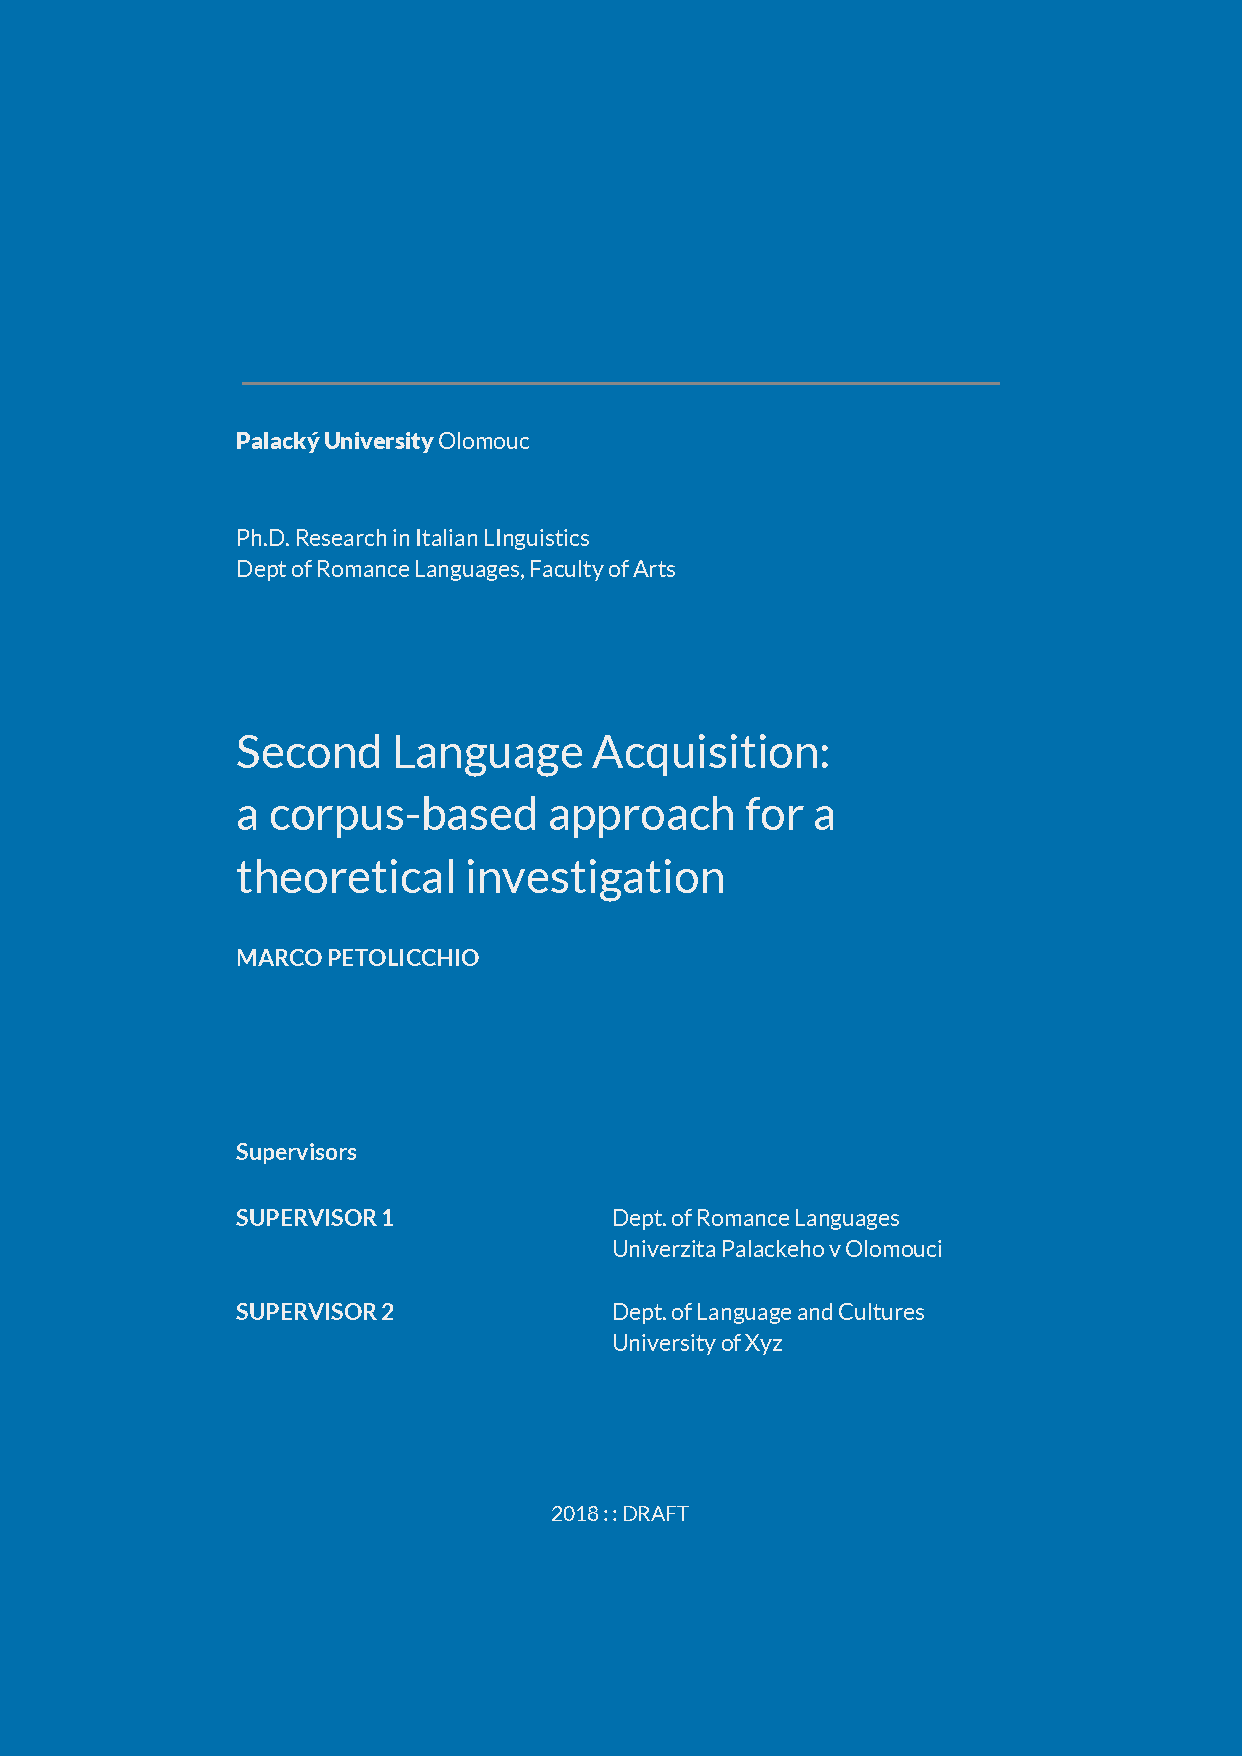
\includepdf{frontmatter.pdf}

{
\setcounter{tocdepth}{1}
\tableofcontents
}
\chapter{Preface}\label{preface}

\section{Abstract}\label{abstract}

The aim of the present PhD research is to analyse in a coherent way the
learning path displayed by Czech learners acquiring the Italian
Language, basing on the evidences which result from the independent
linguistic corpus \href{http://czech-it.github.io}{Czech-IT!}. This
study grows up from the researches in Second Language Acquisition and
wishes to retrieve data from applied fields turning them into theoretic
and formal questions in general linguistics.

\section{Keywords}\label{keywords}

\begin{itemize}
\tightlist
\item
  Computational Linguistics
\item
  Syntax
\item
  Second Language Acquisition
\item
  Italian L2
\item
  Corpus Linguistics
\end{itemize}

\chapter{Introduction}\label{introduction}

The main idea under this PhD proposal moves across the idea of an
empirically-grounded research to investigate the strategies of the
learners during the acquisition of the second languages. My task is
twofold: on one side this provide for the developing of a
theoretically-grounded framework to research in the fields of Second
Language Acquisition (SLA), while on the other this necessitate to
realize a linguistic corpus which collect in a coherent fashion a wide
set of data and facts in order to give a transparent documentation of
the learning path. At the current date, the corpus is actively mantained
online under the name \enquote{Czech-IT!} and counts 220 items by more
than 50 learners \citep{czech-it}. In this order of ideas, the project
is focused around the analysis of Czech and Slovak learners which
acquire the Italian language as L2.

Czech (CZ) is a West Slavic language of the Indoeuropean (IE) family
\citep[\citet{glottolog}]{beekes_comparative_2011}, widespreadly known
for its morphological complexity with a very rich inflectional and
derivational system in the word formation. Italian (IT) is a Romance
language of the IE family, strictly related to Latin\footnote{For the
  sake of clarity: I am going to refer to Italian in its standard
  variety. Cfr.
  \citep[\citet{d_achille-italiano}]{berruto2012sociolinguistica} for a
  general overview of the contemporary IT.} , which exhibits a wide
range of variation in dialects, regional languages and specialistic
styles. Commercial and cultural links between the Czech Republic and
Italy are effective and deep, and the studying of Italian language
amongst native Czech learners is a remarkable fact. This kind of
research is intimately twofold in nature and embraces differences
approaches and discipline: the developing of a linguistic corpus
(digital humanities, corpus and computational linguistics) and a
theoretically-oriented analysis (general and theoretical linguistics,
studies on SLA and interlanguage).

\section{The empirical ground}\label{the-empirical-ground}

By a strictly linguistic analysis, CZ and IT know a set of phenomena
which diverges a while and permits to afford for a comparative
investigation, focused in the errors displayed during the acquisitional
path: the absence of the Determiner phrase (DP) and the rich
morphological declension in the CZ noun syntax, where IT does not
exhibit this kind of morphological complexity and does not permit the
delection of the Determiners in such contexts
\citep[\citet{longobardi-n_movement}]{bianchi-1992}, which gives
examples of omission or ipercorrected forms or examples due to the L1
habits. As a framework-free corpus with no theoretical issues, Czech-IT!
aims to be a resource either for speculative, data-based studies, as
well than for empirically based L2 acquisition teaching processes. The
project and the datasets are licensed under a Creative Commons
Attribution 4.0 International License, for which it represents an open
source and an open data project, in the universe of the \emph{open
knowledge} works. This represent also a tempt to gain indipendence from
data to the analysis of the data itself, creating a linguistic corpus
threated in a computational manner
\citep[\citet{kuebler-corpus_linguistics}, \citet{schmid-treetagger},
\citet{bird-nltk}, \citet{kurdi_natural_2016-2},
\citet{clark_handbook_2010-1}]{abney1997}, in line with other wll
established learner corpora on Italian L2 \citep[\citet{lips}]{valico}.

\subsection{Data}\label{data}

In order to define a wider range of linguistic situations, there are
different kind of linguistic productions in the corpus:

\begin{itemize}
\tightlist
\item
  an email subcorpus for the (quasi-) bureaucratic and academic
  language;
\item
  SMS and other direct platforms for textual messaging for informal
  situations;
\item
  spoken discourse analysis for spontaneous modality;
\item
  some online surveys created for obtaining auto valutation by learners
  about their acquisition: the tests are made by a certain amount of
  questions and tiny writing samples.
\end{itemize}

The data are inserted at first in textual forms, where are stored the
relevant informations about the learner, the date and notes of the
revisor, while the textual content of each relevant example is processed
towards the usage of automatic machinery, which yields syntactical,
morphological and part of speech tagging annotations, relevant for
quantitative and statistical outcomes. Currently, a primary dataset
which contains the items is linked to other two datasheets, one relative
to learners and the other for manual categorization of linguistic
phenomena and automatic treatment of the texts, as for tokenization,
lemmatization and POS-tagging procedures. Separating the raw data from
the annotation scheme seems to be a feasible way to retain data in a
wide output directions, e.g.~for data-visualization outcomes, and can be
effectively implemented towards the successive implementation without
the necessity to rethink the overall platform. Also, it permits to data
to be independent from contingent purposes and easily accessible and
used by the whole community of scholars, researchers, and interested
users. It could be usable for data-driven approaches to learning second
language and for theoretically-oriented researches on interlanguage,
syntactic variation and computational linguistics.

\subsubsection{The learners}\label{the-learners}

Currently, the number of the learners inserted in the dataset is 51:
they are in the most part native-Czech learners but a small part of
Slovak is represented. The level of education testimoniates a
representative range of different kinds of acquisition paths, as well
than the different ages of the learners.

\subsubsection{The texts}\label{the-texts}

At the present date, there are 220 entries in the corpus, which reveal a
large range of different communicative situations, from spontaneous
messages as chat, spoken conversations, and email towards written
homeworks for retrieve targeted hypotheses on the learning way.

\section{The theoretical framework}\label{the-theoretical-framework}

\subsection{Variation in grammar}\label{variation-in-grammar}

From a theoretical viewpoint, the research is inserted in the current
theories which rely on the hierarchical functioning of the language
faculty, for which the variation among languages are reconducted to a
parametrizing of choice among the structures of languages
\citep[\citet{chomsky1998}, \citet{chomsky2013}, \citet{chomsky2015},
\citet{adger2011}, \citet{rizzi2013}]{chomsky1995}. This view permits on
one side to compare the syntactic structures in a coherent and schematic
way, while on the other it concentrates moreover on the hierarchical
fashion of the language faculty than on the linear order displayed by
the utterances.

\subsection{Comparative analyses and the role of the
interlanguage}\label{comparative-analyses-and-the-role-of-the-interlanguage}

The role of the native language (L1) can conditionates deeply the way in
which the target language (L2) is acquired during the learning path: an
emblematic case is the \emph{transfer} of the knowledge about the
structures of the L1 to the target, revealing the interlanguage. During
the last 20 years, a considerable part of linguistic literature is
involved in developing some sort of models to think how the faculty of
language can work, in its biological \citep{hcf2002}, computational
\citep{fodor2001} and cognitive components in a highly interdisciplinary
environment. Studies on SLA is a fertile field, which relies on
comparative and contrastive analyses of linguistic phenomena, either
both from an applied view \citep{ellis_study_101} than by theoretically
grounded perspective focused on Generative framework (GenSLA)
\citep[\citet{rothman_slabakova_2017}, \citet{hawkins2001},
\citet{sorace2011pinning}]{guasti2002}. In this sense appears that the
adoption of a coherent model to analyze the variation in gramar in
parametric model can be suitable for long-standing researches on SLA and
interlanguage, also based on independent data-mining initiatives as in
the case of the present purposes, which disentangles the data in a form
of a linguistic corpus and the linguistic analysis.

\section{Models and methods}\label{models-and-methods}

{[}compLing{]}

A similar project aims to show an affordable platform for linguistic
data-based researches.

The advantage of a such type of way to proceed is twofold: on one side
it permits a clear separation between the data and the investigations of
the data itself, while it offers a theoretically-agnostic way to collect
the data which can be used in a widespread linguistic researches and
model, not confined to some theoretically-oriented approaches. Along
this path, such a kind of corpora can be suited either in academic
enterprises than for private and corporate initiatives, as well in
teaching models in the SLA field, oriented towards an
empirically-grounded perspective on error and interlanguage analyses.
The usage of computational and digital architecture
\citep[\citet{kurdi_natural_2016-2},
\citet{kuebler-corpus_linguistics}]{clark_handbook_2010-1} represents a
standpoint in the current path of linguistic studies, resulting in a
highly interdisciplinary model to researching. The theoretical model
established relies on generative studies to language, applied to a new
and insightful field of research as the SLA studies. It permits to
obtain an empirically-grounded and theoretically coherent perspective on
some pattern displayed during the learning path.

\section{Structure of the project}\label{structure-of-the-project}

\subsection{Roadmap}\label{roadmap}

The first year is dedicated to the setting-up of the corpus, with the
starting operations to acquire the data and elaborate a coherent way to
annotate the texts with a standard schema. During the second year the
corpus is planned to grow up for reach a significance level of
\textgreater{}15000 words in order to provide quantitative analyses.
Third and fourth year will be spent in developing the theoretical
analyses and refining the informatic architecture of the project,
evolving in a user-friendly and interrogable way to dispense the data.
The theoretical outcome constitues the main topic of the research.

\subsection{Thesis structure}\label{thesis-structure}

here at last.

\chapter{Backmatter}\label{backmatter}

\section{Credits}\label{credits}

This project is constituted by files written in Markdown syntax and
exported either as a standalone website both as printer-ready product.
This is due to the awesome work of the people behind different
libraries:

\begin{itemize}
\tightlist
\item
  \href{https://bookdown.org}{Pandoc}
\item
  \href{https://bookdown.org}{Bookdown}
\item
  \href{https://bookdown.org}{RMarkdown} and
  \href{https://bookdown.org}{R} environment.
\end{itemize}

As well, for the computational infrastructure, a lot of open source
tools have been used:

\begin{itemize}
\tightlist
\item
  \href{https://bookdown.org}{NLTK}
\end{itemize}

For the typographic setting, the print-ready file is composed on LaTeX
with the usage of SCRBOOK class and some custom component. I am aware I
can't thank everyone on the web about that. By the way, thank you!

\section{About the author}\label{about-the-author}

I am a Graduate Researcher involved in a Ph.D.~Program in Italian
Linguistics at the Department of Romance Studies in the Faculty of
Phylosophy at Palacky University in Olomouc, Czech Republic.

My interests span across digital humanities, syntax theories and
computational linguistics.

Feel free to write me at
\href{mailto:marco.petolicchio@gmail.com}{\nolinkurl{marco.petolicchio@gmail.com}}
or visit marcopetolicchio.com for the detailed contact list.

\bibliography{bibliography.bib}

\listoftables
\listoffigures


\clearpage
\chapter*{Timestamp}
\vfill
\begin{center}

Printed on: \today

\end{center}

\end{document}
